
\documentclass{article}

\usepackage{graphicx}
\usepackage{hyperref}
\usepackage{tikz}

\title{Projet programmation 2\\Phase 2}
\author{R\'emi Oudin, Alexis Laouar, K\'evin Le Run}
\date{}

\begin{document}

\maketitle

\section{Types d'ennemis}

\begin{itemize}

\item 
\includegraphics{bunny_alt1.png} \texttt{Lapin normal}

L'ennemi de base, se d\'eplace \`a vitesse moyenne.

\item 
\includegraphics{hare_alt1.png} \texttt{Li\`evre}

Le li\`evre est tr\`es rapide mais poss\`ede peu de points de vie.

\item 
\includegraphics{bunny_alt1.png} \texttt{Lapin lourd}

Ce lapin, tr\`es lent, poss\`ede beaucoup de points de vie.

\item 
\includegraphics{badassbunny.png} \texttt{Lapin badass}

Ce lapin poss\`ede beaucoup de points de vie et donne naissance \`a des lapins
normaux \`a sa mort.

\item 
\includegraphics{shield_bunny.png} \texttt{Lapin Bouclier}

Ce lapin augmente le bouclier des lapins avoisinants.

\item 
\includegraphics{ninja.png} \texttt{Lapin SpecOps/Lapin Ninja}

Ce lapin est capable de se t\'el\'eporter.

\item 
\includegraphics{otter.png} \texttt{Loutre}

La loutre est le premier (et pour l'instant seul) boss du jeu. Elle a beaucoup
de points de vie mais est tr\`es lente.

\item 
\includegraphics{goldenbunny_alt1.png} \texttt{Lapin dor\'e}

Ce lapin tr\`es rare et tr\`es rapide rapporte beaucoup d'or si \'elimin\'e.

\end{itemize}

\section{Types de tours}

\begin{itemize}

\item 
\includegraphics{base_tower.png} \texttt{Lance-carrotes}

Cette tour tire une carotte sur l'ennemi le plus avanc\'e.

\item 
\includegraphics{quick_tower.png} \texttt{Mitrailleuse}

Cette tour tire des feuilles (tr\`es l\'eg\`eres mais peu dangereuses) \`a
tr\`es grande vitesse et en tr\`es grande quantit\'e.

\item 
\includegraphics{tank.png} \texttt{Tour lourde}

Cette tour tire des carottes transg\'eniques tr\`es lourdes qui causent
beaucoup de d\'egats aux ennemis.

\item 
\includegraphics{heavy_tower.png} \texttt{\'Epouvantail}

Cette tour tire simultan\'ement sur tous les ennemis \`a port\'ee.

\item 
\includegraphics{base_tower.png} \texttt{Catapulte \`a navet}

Cette tour lance des navets explosifs sur les ennemis \`a port\'ee.

\item 
\includegraphics{roberto.png} \texttt{Roberto}

Roberto est un soldat psychique enferm\'e dans une capsule en verre capable
d'attaquer les ennemis \`a distance.

\item 
\includegraphics{roberto.png} \texttt{Acc\'el\'erateur d'entropie}

Cette tour g\`ele les alentours, ralentissant les ennemis dans la zone.

\item 
\includegraphics{radar.png} \texttt{Ing\'enieur}

Cette tour augmente les d\'egats des tours avoisinantes.

\end{itemize}

\section{Plus court chemin}

L'algorithme que nous avons choisi afin de d\'eterminer un chemin pours les
ennemis est
\href{http://users.cecs.anu.edu.au/~dharabor/data/papers/harabor-grastien-aaai11.pdf}
{Jump Point Search} (JPS).

JPS est un algorithme qui optimize la recherche de chemin de A* en ajoutant
\`a la recherche  l'information de direction, \'eliminant une grande quantit\'e
de noeuds ouverts.

\begin{figure}[h]
    \centering
    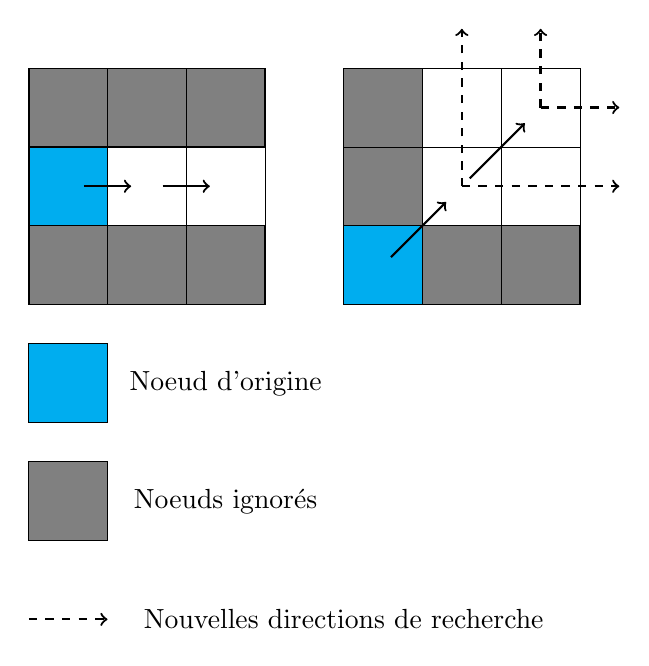
\begin{tikzpicture}
        \draw[fill=cyan] (0,1) rectangle (1,2);
        \draw[fill=gray] (0,0) rectangle (3,1);
        \draw[fill=gray] (0,2) rectangle (3,3);
        \draw[step=1cm,very thin] (0,0) grid (3,3);
        \draw[thick,->] (1.7,1.5) -- (2.3,1.5);
        \draw[thick,->] (0.7,1.5) -- (1.3,1.5);

        \draw[fill=cyan] (4,0) rectangle (5,1);
        \draw[fill=gray] (4,1) rectangle (5,3);
        \draw[fill=gray] (5,0) rectangle (7,1);
        \draw[step=1cm,very thin] (4,0) grid (7,3);
        \draw[thick,->] (4.6,0.6) -- (5.3,1.3);
        \draw[thick,->] (5.6,1.6) -- (6.3,2.3);
        \draw[thick,dashed,->] (5.5,1.5) -- (5.5,3.5);
        \draw[thick,dashed,->] (5.5,1.5) -- (7.5,1.5);
        \draw[thick,dashed,->] (6.5,2.5) -- (6.5,3.5);
        \draw[thick,dashed,->] (6.5,2.5) -- (7.5,2.5);

        \draw[black,fill=cyan] (0,-0.5) rectangle (1,-1.5);
        \node at (2.5,-1) {Noeud d'origine};
        \draw[black,fill=gray] (0,-2) rectangle (1,-3);
        \node at (2.5,-2.5) {Noeuds ignor\'es};
        \draw[dashed,thick,->] (0,-4) -- (1,-4);
        \node at (4,-4) {Nouvelles directions de recherche};
    \end{tikzpicture}
    \caption{Beaucoup de cases ignor\'ees}
\end{figure}

\newpage
Lorsqu'un obstacle rompt l'hypoth\`ese que les noeuds adjacents ne sont pas
atteint de mani\`ere optimale depuis le noeud actuel, on a atteint un Jump
Point.

\begin{figure}[h]
    \centering
    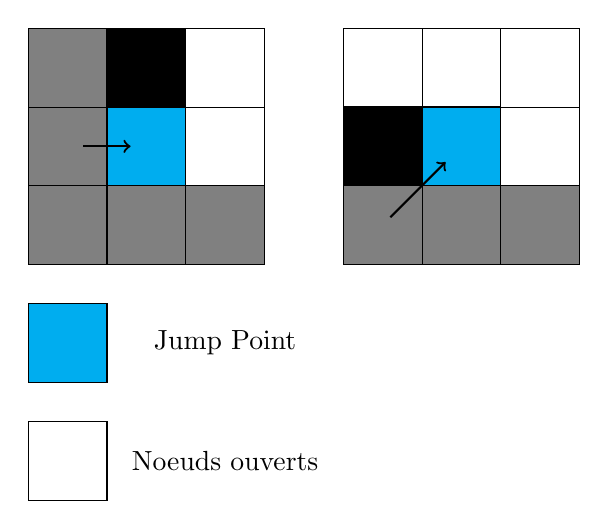
\begin{tikzpicture}
        \draw[fill=cyan] (1,1) rectangle (2,2);
        \draw[fill=gray] (0,0) rectangle (1,3);
        \draw[fill=gray] (1,0) rectangle (3,1);
        \draw[fill=black] (1,2) rectangle (2,3);
        \draw[step=1cm,very thin] (0,0) grid (3,3);
        \draw[thick,->] (0.7,1.5) -- (1.3,1.5);

        \draw[fill=cyan] (5,1) rectangle (6,2);
        \draw[fill=black] (4,1) rectangle (5,2);
        \draw[fill=gray] (4,0) rectangle (7,1);
        \draw[step=1cm,very thin] (4,0) grid (7,3);
        \draw[thick,->] (4.6,0.6) -- (5.3,1.3);

        \draw[black,fill=cyan] (0,-0.5) rectangle (1,-1.5);
        \node at (2.5,-1) {Jump Point};
        \draw[black] (0,-2) rectangle (1,-3);
        \node at (2.5,-2.5) {Noeuds ouverts};
    \end{tikzpicture}
    \caption{Les Jump Points}
\end{figure}

\end{document}
